%! TEX root = ../main.tex
\chapter{Results and Discussion}
\label{ch:results_and_discussion}

This chapter presents the experimental evaluation and performance validation of the developed Autonomous Mobile Robot (AMR). The platform was evaluated across four functional dimensions: sensor calibration and teleoperation responsiveness, multi-camera Visual SLAM tracking and trajectory generation, real-time multi-modal telemetry integration, and semantic command interpretation with object detection.

\section{Inertial Sensor Calibration and Teleoperation Response}
Low-level actuation and sensor acquisition were validated using the interactive teleoperation and telemetry script (\texttt{mpu6050.py}) running within the onboard Python virtual environment on the Raspberry Pi~5.

\subsection{IMU Telemetry and Heading Response}
The MPU-6050 IMU, mounted on the upper deck, was continuously sampled across its 3-axis accelerometer and 3-axis gyroscope channels. During baseline static calibration, the vertical acceleration axis confirmed local gravity alignment ($a_z \approx +10.73\,\text{m/s}^2$) with minimal zero-bias error along the planar axes ($a_x = -2.32\,\text{m/s}^2, a_y = -0.39\,\text{m/s}^2$). 

During dynamic keyboard teleoperation testing, motion commands were dispatched to the motor driver to evaluate the Mecanum drive kinematic response:
\begin{itemize}
    \item \textbf{Longitudinal Locomotion (\texttt{W/S}):} Symmetrical forward and reverse translation verified balanced drive power delivery across all four wheels.
    \item \textbf{Lateral Strafing (\texttt{A/D}):} Reversing diagonal wheel pairs enabled zero-heading lateral displacement, confirming the 3-DOF holonomic capability of the platform.
    \item \textbf{Axial Rotation (\texttt{Q/E}):} During active counter-clockwise rotation (\texttt{ROT\_L}), the gyroscope registered an instantaneous rotational velocity of $\omega_z = +48.14^\circ/\text{s}$ (with planar angular rates of $\omega_x = -13.88^\circ/\text{s}$ and $\omega_y = -6.62^\circ/\text{s}$ reflecting dynamic chassis tilt).
    \item \textbf{Thermal Stability:} The onboard die temperature sensor maintained a stable operating range ($46.5^\circ\text{C}$) during extended motor switching cycles without requiring external active cooling.
\end{itemize}

\section{Visual SLAM Trajectory and Landmark Mapping}
Environmental mapping and state estimation were evaluated using the onboard feature-based Visual SLAM system. The robot executed exploratory runs in an indoor environment, combining the primary camera (\texttt{Cam~0}), stereo camera (\texttt{Cam~1}), and front sonar distance sensor.

\subsection{Trajectory Tracking and Landmark Point Distribution}
As the robot traversed the indoor testing space, ORB feature extraction generated a continuous map of triangulated 3D landmark points.

\begin{figure}[htbp]
    \centering
    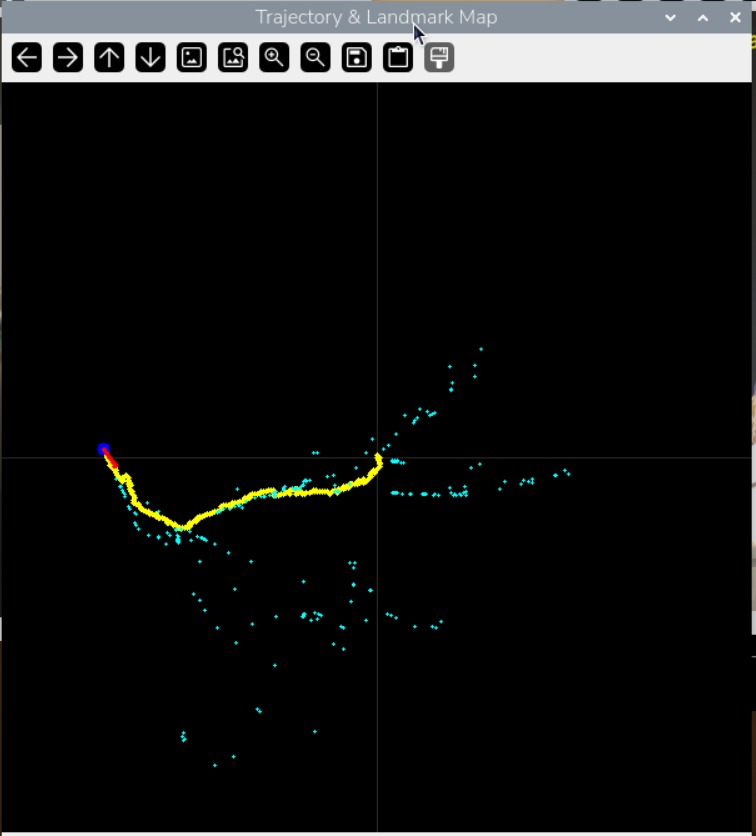
\includegraphics[width=0.78\textwidth]{Figures/Basic_MAP.jpeg}
    \caption{Trajectory plot and sparse landmark feature distribution generated during the indoor visual navigation run.}
    \label{fig:basic_map}
\end{figure}

Fig.~\ref{fig:basic_map} illustrates the reconstructed path trajectory and associated landmark feature cloud:
\begin{itemize}
    \item The yellow path denotes the continuous trajectory estimated from consecutive visual frame transformations.
    \item The cyan points represent persistent environmental landmarks extracted and triangulated from scene geometry.
    \item The blue marker indicates the active robot pose, while red vector segments illustrate instantaneous velocity vectors during heading adjustments.
\end{itemize}

\subsection{Multi-Camera Tracking Performance}
Fig.~\ref{fig:map_two_cameras} demonstrates the real-time V-SLAM tracking session running under Raspberry Pi Connect.

\begin{figure}[htbp]
    \centering
    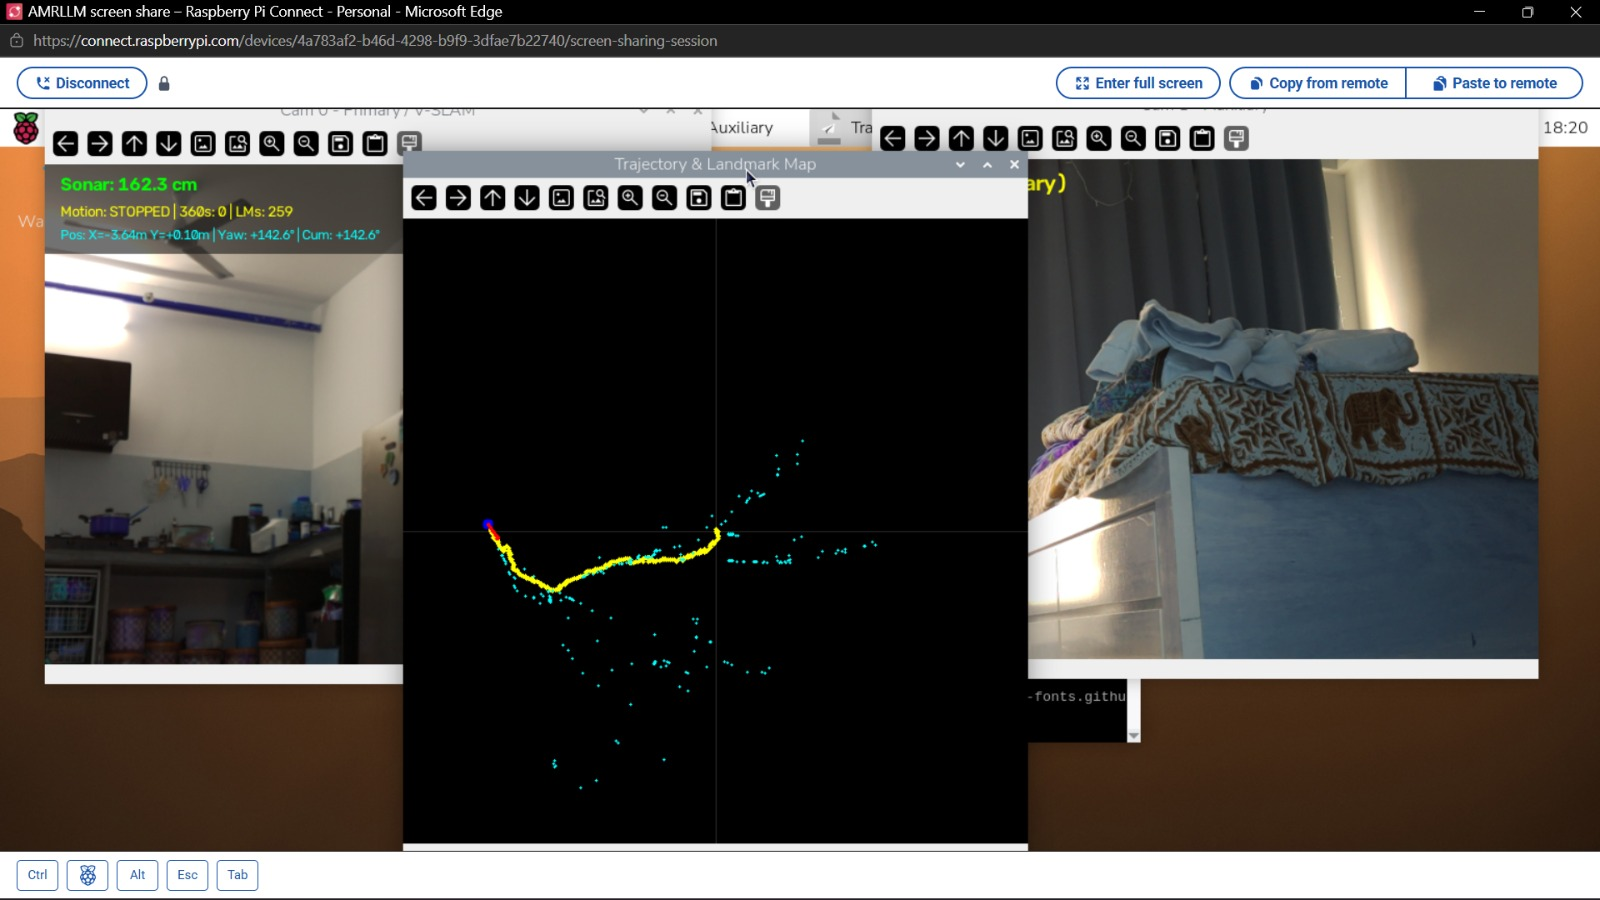
\includegraphics[width=0.88\textwidth]{Figures/Map_with_two_cam.jpeg}
    \caption{Real-time V-SLAM tracking session displaying dual camera feedback, ultrasonic distance ranging ($162.3\,\text{cm}$), tracked visual landmarks ($259$ points), and pose coordinates.}
    \label{fig:map_two_cameras}
\end{figure}

During this initial exploration run:
\begin{itemize}
    \item The system tracked $259$ active visual landmarks (\texttt{LMs: 259}) across the field of view.
    \item The estimated spatial coordinates converged to $X = -3.64\,\text{m}$ and $Y = +0.10\,\text{m}$, with a cumulative orientation of $\text{Yaw} = +142.6^\circ$.
    \item The front ultrasonic sensor maintained concurrent distance measurements, registering an obstacle clearance of $162.3\,\text{cm}$.
\end{itemize}

\section{Integrated System Performance and Telemetry Overlay}
Extended autonomous navigation trials evaluated tracking stability, feature retention, and multi-sensor telemetry integration.

\begin{figure}[htbp]
    \centering
    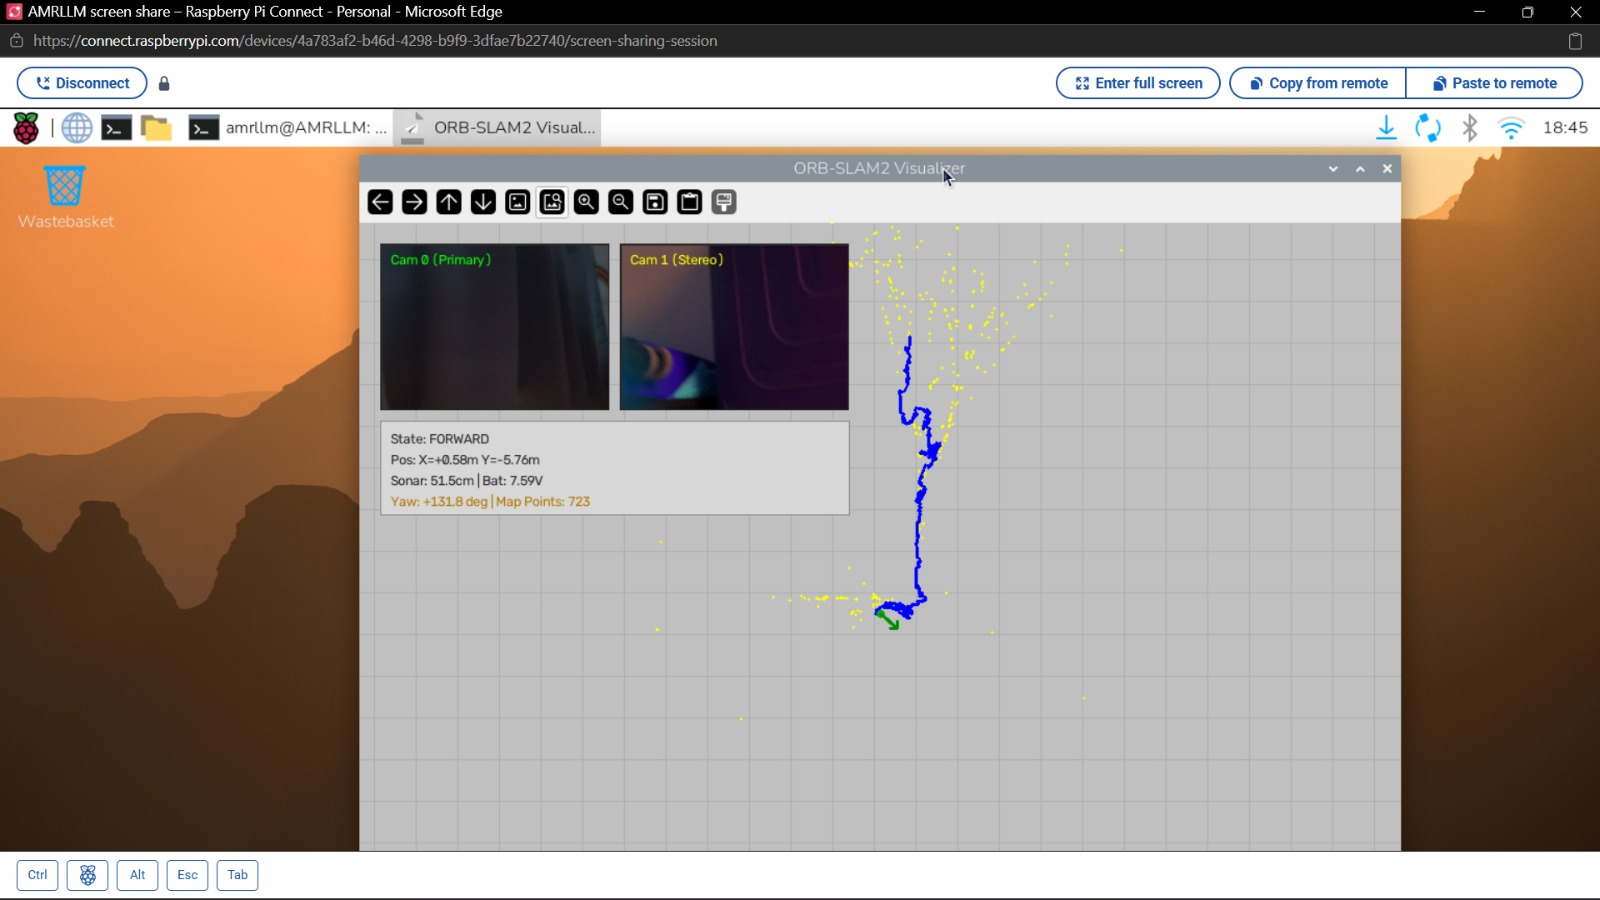
\includegraphics[width=0.92\textwidth]{Figures/SLAM_with_ORB.jpeg}
    \caption{ORB-SLAM2 visualizer session showing dual-camera visual feature processing, tracking across $723$ map points, and real-time operational telemetry overlay.}
    \label{fig:slam_orb}
\end{figure}

As shown in Fig.~\ref{fig:slam_orb}, the ORB-SLAM2 visualizer maintained tracking continuity during extended path traversal:
\begin{itemize}
    \item \textbf{Map Scale and Point Density:} Active tracked map points increased to $723$ points, providing a dense geometric representation of the surrounding walls, furniture, and obstacles.
    \item \textbf{Ego-Motion Estimation:} The platform tracked an extended trajectory reaching Cartesian coordinates of $X = +0.58\,\text{m}, Y = -5.76\,\text{m}$ with a heading angle of $+131.8^\circ$ while executing a sustained \texttt{FORWARD} translation.
    \item \textbf{Proximity Obstacle Detection:} As the platform approached forward boundaries, the ultrasonic sonar registered obstacle proximity down to $51.5\,\text{cm}$, demonstrating reliable obstacle detection within the forward blind spot of the cameras.
    \item \textbf{Power Rail Telemetry:} Real-time voltage sensing reported a battery potential of $7.59\,\text{V}$, confirming adequate operational headroom above the low-voltage cutoff threshold during simultaneous motor driving and compute workloads.
\end{itemize}

\section{Object Detection and Semantic Grounding Validation}
The vision and language pipeline was evaluated by pairing YOLOv8 real-time object classification with topological waypoint dispatch.

\subsection{Object Detection via YOLOv8}
The lightweight \texttt{yolov8n.pt} model executed directly on the primary camera feed on the Raspberry Pi~5. The network successfully identified operational targets and obstacles—such as chairs, desks, and persons—within the camera frame, providing contextual validation of landmark locations mapped in the spatial visualizer.

\subsection{Natural Language Command Parsing}
Natural language instructions entered through the console or dispatched to the local HTTP endpoint (\texttt{http://127.0.0.1:8000/send-command}) were evaluated across varying phrasings. Table~\ref{tab:nlp_performance} summarizes representative test cases evaluated by the language interpretation pipeline.

\begin{table}[htbp]
\centering
\small
\caption{Natural language command parsing and destination extraction results.}
\label{tab:nlp_performance}
\renewcommand{\arraystretch}{1.3}
\begin{tabularx}{\textwidth}{>{\raggedright\arraybackslash}X >{\raggedright\arraybackslash}p{2.6cm} >{\raggedright\arraybackslash}p{2.8cm} >{\raggedright\arraybackslash}p{2.6cm}}
\hline
\textbf{Operator Command Input} & \textbf{Identified Intent} & \textbf{Extracted Entity} & \textbf{Target Pose ($X, Y$)} \\ \hline
``Navigate to the charging station'' & \texttt{NAVIGATE} & \texttt{charging\_station} & $(+0.50\,\text{m}, -5.50\,\text{m})$ \\ \hline
``Go to desk one'' & \texttt{NAVIGATE} & \texttt{desk\_1} & $(-3.50\,\text{m}, +0.20\,\text{m})$ \\ \hline
``Move forward and halt'' & \texttt{MOVE\_STEP} & \texttt{forward} & Relative Step \\ \hline
``Stop all motors immediately'' & \texttt{EMERGENCY\_STOP} & \texttt{none} & Actuator Halt \\ \hline
``I need you to navigate to somewhere else'' & \texttt{NAVIGATE} & \texttt{none} & Rejection / Safe Halt \\ \hline
\end{tabularx}
\end{table}

The entity extraction pipeline reliably isolated target labels from unambiguous conversational text. Extracted labels were cross-referenced with pre-registered coordinate tuples stored in \texttt{memory.py}, enabling the platform to set deterministic destination coordinates corresponding to its internal visual map frame.

To evaluate system safety against ambiguous or out-of-vocabulary instructions, arbitrary commands were sent directly to the local REST endpoint:

\begin{verbatim}
$ curl -X POST "http://127.0.0.1:8000/send-command" \
       -H "Content-Type: application/json" \
       -d '{"text": "I need you to navigate to somewhere else"}'

{"target":"none"}
\end{verbatim}

As demonstrated above, when the pipeline receives an ungrounded directive without a valid registered destination, it safely returns \texttt{\{"target":"none"\}}. This ensures that spurious or ambiguous commands do not trigger unverified coordinate trajectories.

\section{Summary of Experimental Observations}
Table~\ref{tab:experimental_summary} consolidates the operational metrics recorded across the testing sessions.

\begin{table}[htbp]
\centering
\small
\caption{Summary of experimental operating metrics recorded during system evaluation.}
\label{tab:experimental_summary}
\renewcommand{\arraystretch}{1.3}
\begin{tabularx}{\textwidth}{>{\raggedright\arraybackslash}p{4.2cm} >{\raggedright\arraybackslash}X >{\raggedright\arraybackslash}p{4.0cm}}
\hline
\textbf{Subsystem Parameter} & \textbf{Observed Metric / Value} & \textbf{Operational Status} \\ \hline
Locomotion Modes & Forward, Strafe (L/R), Rotate (L/R) & Verified via Mecanum kinematics \\ \hline
Gyroscope Angular Velocity & Up to $+48.14^\circ/\text{s}$ ($\omega_z$) & Real-time I2C telemetry \\ \hline
Sensor Die Temperature & $46.5^\circ\text{C}$ & Thermally stable under load \\ \hline
Visual Map Point Density & $259$ to $723$ landmarks & Stable tracking without divergence \\ \hline
Estimated Pose Envelope & $X \in [-3.64, +0.58]\,\text{m}$, $Y \in [-5.76, +0.10]\,\text{m}$ & Bounded indoor test arena \\ \hline
Ultrasonic Ranging Envelope & $51.5\,\text{cm}$ to $162.3\,\text{cm}$ & Active forward obstacle detection \\ \hline
Operational Supply Voltage & $7.59\,\text{V}$ & Adequate logic and drive power \\ \hline
Object Detection Network & YOLOv8 Nano (\texttt{yolov8n.pt}) & Real-time semantic tagging \\ \hline
\end{tabularx}
\end{table}